\documentclass[12pt,a4paper,oneside]{report}

\usepackage[utf8]{inputenc}
\usepackage[T1]{fontenc}
\usepackage{lmodern}
\usepackage{microtype}
\usepackage{geometry}
\usepackage{setspace}
\usepackage{graphicx}
\usepackage{booktabs}
\usepackage{array}
\usepackage{amsmath}
\usepackage{amssymb}
\usepackage{siunitx}
\usepackage{hyperref}
\usepackage{xcolor}
\usepackage{caption}
\usepackage{subcaption}
\usepackage{longtable}

\geometry{margin=2.7cm}
\onehalfspacing
\graphicspath{{figures/}}
\hypersetup{
  colorlinks=true,
  linkcolor=blue!45!black,
  citecolor=blue!45!black,
  urlcolor=blue!45!black
}
\sisetup{detect-all=true}

\title{
  \vspace{1.5cm}
  \textbf{Thermodynamic Phase Stability and Local Database Workflows for Cu/Ga Bulk and Surface Structures}\\[0.5cm]
  \large A Computational Chemistry Master Thesis Based on OnePiece, ASE and pandas DataFrames
}
\author{Codex}
\date{\today}

\begin{document}

\maketitle

\begin{abstract}
This thesis investigates a local computational chemistry dataset of Cu/Ga bulk,
oxide-derived bulk, cluster and surface structures stored as pandas HDF files.
The dataset combines density-functional-theory-derived energies, relaxed atomic
structures, geometric descriptors, Bader-like charge descriptors, surface
coverages, reference energies and thermodynamic correction terms. The work has
two connected aims. First, it develops a reproducible analysis of bulk and
surface phase stability as a function of temperature and the gas ratio
$p_{\mathrm{H_2O}}/p_{\mathrm{H_2}}$. Second, it designs a local user-interface
workflow for browsing, filtering, reviewing and reusing such atomistic data in
a way that resembles high-quality materials databases while remaining entirely
local and file-based.

The computational workflow is implemented in Python with pandas, NumPy, SymPy,
ASE and Plotly/Matplotlib. The input consists of eight HDF files containing 274
calculation records and 90 original columns. Additional context columns are
derived for record type, reference role, phase labels, quality flags, atom
counts and phase-diagram usage. Bulk stability is evaluated by converting
symbolic free-energy expressions to numerical functions over a grid of
temperature and $\log_{10}(p_{\mathrm{H_2O}}/p_{\mathrm{H_2}})$. Surface
stability is evaluated by correcting surface free energies with chemical
potential terms and comparing candidates per surface area. The resulting phase
fields identify stable Cu-rich, intermediate Cu/Ga and Ga-rich regions in the
chosen thermodynamic window. Individual Miller-index analyses show distinct
surface-stability regions for $(100)$, $(110)$, $(111)$ and $(211)$ surfaces.

The thesis also presents PFUI, a local Python package prototype for a materials
database front end. PFUI treats OnePiece-like data objects, HDF files and
pandas DataFrames as interchangeable sources, displays ASE-aware records,
supports image-path columns, and introduces a Controlroom tab for filtering,
row inclusion states, reference discovery and command-like notebook operations.
This combination of computational analysis and interface design provides a
reproducible foundation for future adsorption-energy workflows in which clean
surface references and adsorbate references are resolved directly from the
local dataset.
\end{abstract}

\tableofcontents
\listoffigures
\listoftables

\chapter{Introduction}

The analysis of alloy surfaces is central to modern computational chemistry,
heterogeneous catalysis and materials design. Copper--gallium systems are
particularly interesting because surface enrichment, oxide-derived
thermodynamics and adsorbate binding may all change with temperature, gas
composition and surface orientation. A single relaxed structure is therefore
rarely sufficient. Instead, meaningful interpretation requires a database of
bulk, surface, reference and candidate calculations that can be filtered,
compared and transformed into thermodynamic observables.

Large public platforms such as the Materials Project and OQMD demonstrate how
valuable searchable materials databases can be. In a research project, however,
data often exists first as local calculation folders, HDF files and notebooks.
The scientific problem is then not only to compute a phase diagram, but to make
the data workflow auditable: which rows were used, which calculations were
excluded, which reference surface was selected, which energy expression was
evaluated, and which notebook or script produced a figure.

This thesis addresses that local workflow. The dataset studied here was exported
from a OnePiece-like computational chemistry package into pandas HDF files. The
files contain energies, ASE atomic structures, formulas, surface descriptors,
chemical potentials and derived thermodynamic quantities. The central scientific
task is to construct Cu/Ga phase diagrams as functions of temperature and the
water/hydrogen gas ratio. The central software task is to design an interface
that allows the same calculations to be inspected, filtered and repeated
without forcing the user to edit notebook code for every question.

\section{Research Questions}

The thesis is guided by four questions:

\begin{enumerate}
  \item[\textbf{Q1.}] How can OnePiece HDF files be represented as a chemically meaningful
  pandas DataFrame while preserving provenance and structure context?
  \item[\textbf{Q2.}] Which bulk and surface phases are stable in a thermodynamic window
  defined by $T$ and $p_{\mathrm{H_2O}}/p_{\mathrm{H_2}}$?
  \item[\textbf{Q3.}] Which column profiles and derived descriptors are needed for different
  local database pages such as overview, surface stability, phase diagrams,
  reference matching and quality control?
  \item[\textbf{Q4.}] How can notebook commands be translated into an efficient local user
  interface for filtering, excluding and exporting database rows?
\end{enumerate}

\section{Contributions}

The main contributions are:

\begin{itemize}
  \item a reproducible pandas/ASE workflow for reading and combining Cu/Ga HDF
  files;
  \item tutorial notebooks explaining the workflow for chemistry students with
  Excel-level table experience;
  \item bulk and surface phase diagrams across temperature and gas ratio;
  \item a local Streamlit-based PFUI prototype with a Controlroom tab;
  \item a column-profile system that selects relevant columns for different
  scientific pages;
  \item a foundation for future adsorption-energy calculations based on
  automatic reference matching through row names and structure metadata.
\end{itemize}

\chapter{Theoretical Background}

\section{Density Functional Theory and Atomistic Databases}

The electronic energies in the dataset originate from density functional theory
(DFT), in which the electronic many-body problem is mapped to an effective
single-particle problem through the electron density. The Kohn--Sham formalism
provides the practical foundation for most modern DFT calculations
\cite{kohn1965self}. In typical surface and alloy studies, the exchange
correlation functional is approximated, for example with a generalized gradient
approximation such as PBE \cite{perdew1996generalized}.

For this thesis, the exact electronic-structure input settings are treated as
part of the provenance stored in the local database. The important point is that
the DFT calculations produce total energies, relaxed atomic structures and
diagnostic quantities such as residual forces. These values are then reorganized
into a DataFrame for chemical analysis.

\section{Formation Energies}

For a bulk alloy phase containing $n_{\mathrm{Cu}}$ copper atoms and
$n_{\mathrm{Ga}}$ gallium atoms, a formation energy can be written in a generic
form as
\begin{equation}
  \Delta E_\mathrm{form}
  =
  E_{\mathrm{Cu}_x\mathrm{Ga}_y}
  -
  n_{\mathrm{Cu}}\mu_{\mathrm{Cu}}
  -
  n_{\mathrm{Ga}}\mu_{\mathrm{Ga}}.
\end{equation}
The dataset contains several formation-energy variants, including per-atom,
per-alloy and per-volume forms. The phase-diagram workflow uses
\texttt{formation\_energy\_per\_atom} for the bulk analysis. Some entries are
plain numerical values, while others are symbolic expressions containing
temperature, gas pressure terms and molecular reference quantities.

\section{Oxygen Chemical Potential}

The gas-dependent thermodynamic correction is expressed through an effective
oxygen chemical potential based on the water/hydrogen ratio:
\begin{equation}
  \mu_O =
  E_{\mathrm{H_2O}} - E_{\mathrm{H_2}}
  - T(S_{\mathrm{H_2O}} - S_{\mathrm{H_2}})
  + k_B T \ln\left(\frac{p_{\mathrm{H_2O}}}{p_{\mathrm{H_2}}}\right).
  \label{eq:muO}
\end{equation}
The notebooks use
\begin{align}
  E_{\mathrm{H_2}} &= -6.737~\mathrm{eV},\\
  E_{\mathrm{H_2O}} &= -12.062~\mathrm{eV},\\
  S_{\mathrm{H_2}} &= 1.5044\times 10^{-3}~\mathrm{eV~K^{-1}},\\
  S_{\mathrm{H_2O}} &= 2.2198\times 10^{-3}~\mathrm{eV~K^{-1}},\\
  k_B &= 8.617333262145\times 10^{-5}~\mathrm{eV~K^{-1}}.
\end{align}
The plotted vertical axis is
$\log_{10}(p_{\mathrm{H_2O}}/p_{\mathrm{H_2}})$, whereas
Equation~\ref{eq:muO} uses the natural logarithm. Therefore, the numerical workflow
converts
\begin{equation}
  \ln\left(\frac{p_{\mathrm{H_2O}}}{p_{\mathrm{H_2}}}\right)
  =
  \ln(10)\log_{10}\left(\frac{p_{\mathrm{H_2O}}}{p_{\mathrm{H_2}}}\right).
\end{equation}

\section{Surface Free Energies}

For surfaces, energies must be normalized by area and corrected by reference
chemical potentials. The working expression used for the surface diagrams is
\begin{equation}
  G_\mathrm{surf}^{\mathrm{corr}}
  =
  \frac{
    G_\mathrm{stored}
    + \Delta n_{\mathrm{Ga}}(\mu_{\mathrm{Ga}}^\mathrm{ref}-\mu_{\mathrm{Ga}})
    + \Delta n_{\mathrm{Cu/Zn}}(\mu_{\mathrm{Cu/Zn}}^\mathrm{ref}-\mu_{\mathrm{Cu/Zn}})
  }{A}.
  \label{eq:surfaceG}
\end{equation}
Here $A$ is the surface area. The exact column names in the dataset include
\texttt{form\_G}, \texttt{Area}, \texttt{delta\_Ga}, \texttt{delta\_Cu},
\texttt{delta\_Zn}, \texttt{mu\_Ga}, \texttt{mu\_Cu} and \texttt{mu\_Zn}.

\chapter{Data and Software Infrastructure}

\section{Input HDF Files}

The local Cu/Ga dataset consists of eight HDF files loaded with
\texttt{pd.read\_hdf(filename, key="df")}. They include bulk, oxide-derived
bulk, cluster and individual surface datasets. After combination, the working
cache contains 274 rows and 90 original columns. The row distribution is shown
in Figure~\ref{fig:dataset-counts}.

\begin{figure}[htbp]
  \centering
  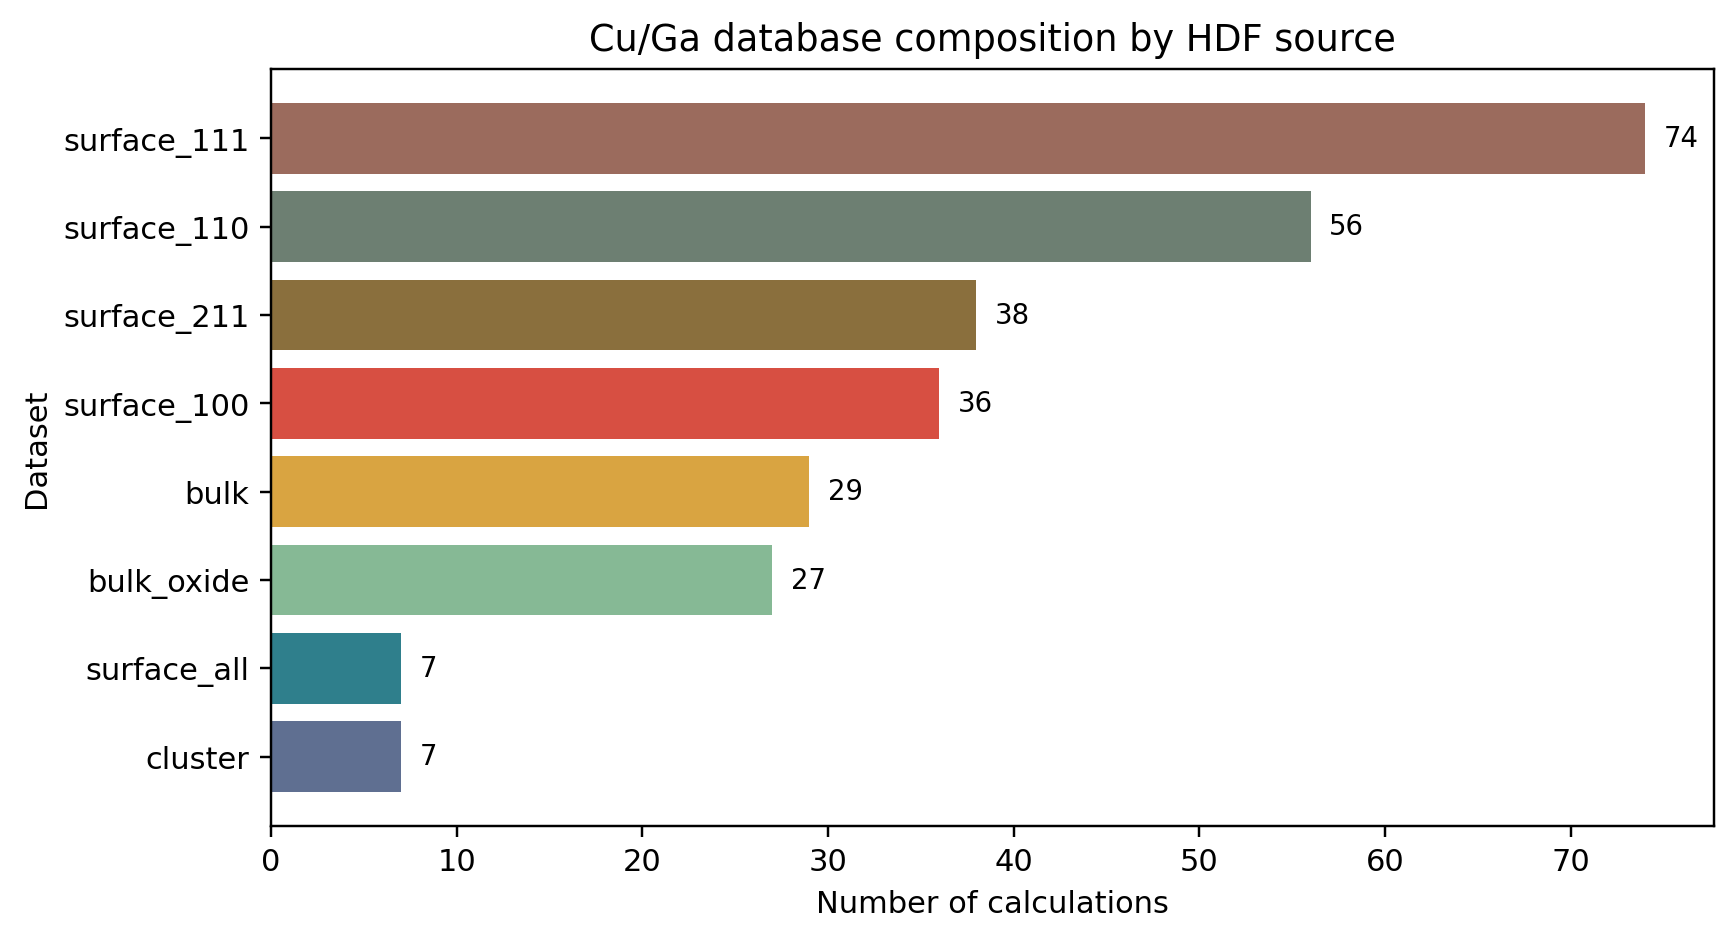
\includegraphics[width=0.82\textwidth]{dataset_counts.png}
  \caption{Number of calculation records per HDF source in the combined Cu/Ga
  dataset.}
  \label{fig:dataset-counts}
\end{figure}

\begin{table}[htbp]
  \centering
  \caption{Summary of the combined local Cu/Ga database.}
  \label{tab:dataset-summary}
  \begin{tabular}{lrrr}
    \toprule
    Dataset & Rows & Unique formulas & Mean $f_\mathrm{max}$ \\
    \midrule
    bulk & 29 & 24 & 0.0066 \\
    bulk\_oxide & 27 & 22 & 0.0045 \\
    cluster & 7 & 1 & 0.0079 \\
    surface\_100 & 36 & 30 & 0.0071 \\
    surface\_110 & 56 & 37 & 0.0070 \\
    surface\_111 & 74 & 33 & 0.0064 \\
    surface\_211 & 38 & 30 & 0.0073 \\
    surface\_all & 7 & 1 & 0.0079 \\
    \bottomrule
  \end{tabular}
\end{table}

\section{Python Data Model}

The workflow uses pandas DataFrames as the central data representation
\cite{mckinney2010pandas}. Each row corresponds to one calculation record, and
columns store energies, formulas, atom counts, structure objects, reference
paths and descriptors. ASE provides the atomistic structure representation
\cite{hjorth2017ase}. NumPy is used for numerical arrays and grid evaluation
\cite{harris2020array}, and Matplotlib/Plotly are used for figures and
interactive surfaces \cite{hunter2007matplotlib}.

Several derived columns are added for UI and analysis:
\begin{itemize}
  \item \texttt{row\_uid}: stable identifier based on HDF source and source row;
  \item \texttt{record\_type}: bulk, surface, cluster or generic record;
  \item \texttt{is\_clean}: whether the row appears to be a clean reference;
  \item \texttt{is\_adsorbate\_like}: whether the name suggests an adsorbate;
  \item \texttt{reference\_role}: candidate, clean surface reference, bulk
  reference or adsorbate candidate;
  \item \texttt{n\_atoms}, \texttt{energy\_per\_atom} and
  \texttt{quality\_flag}.
\end{itemize}

\section{Tutorial Notebooks}

The thesis figures are derived from the tutorial notebooks and scripts created
for this project:
\begin{itemize}
  \item \texttt{cuga\_muO\_temperature\_phase\_diagram.ipynb};
  \item \texttt{00\_hdf\_onepiece\_pandas\_ase\_intro.ipynb};
  \item \texttt{01\_bulk\_phase\_table\_from\_hdf.ipynb};
  \item \texttt{02\_surface\_phase\_tables\_from\_hdf.ipynb};
  \item \texttt{03\_multiplot\_transition\_tables.ipynb}.
\end{itemize}
The notebooks are intentionally written as teaching material for chemists who
are familiar with tables from Excel but are still learning pandas.

\chapter{Methods}

\section{Data Loading and Cleaning}

The HDF files are read into pandas and concatenated into a single local cache.
Three provenance columns are inserted:
\texttt{dataset}, \texttt{source\_hdf} and \texttt{source\_row}. These columns
ensure that every row in a derived plot can be traced back to the original HDF
source.

Some columns contain mixed types. For example,
\texttt{formation\_energy\_per\_atom} can contain a number in one row and a
symbolic expression in another. This is chemically meaningful but challenging
for generic table renderers. Therefore, numerical versions such as
\texttt{formation\_energy\_per\_atom\_numeric} are derived where possible while
the symbolic text is preserved for auditability.

\section{Quality Screening}

The maximum residual force \texttt{fmax} is used as a simple relaxation-quality
indicator. The distribution is shown in Figure~\ref{fig:fmax}. The practical UI
threshold used in the Controlroom is $f_\mathrm{max}<0.05~\mathrm{eV/A}$ for
quick screening. This threshold is not a universal physical law; it is a local
review rule that can be adjusted by the user.

\begin{figure}[htbp]
  \centering
  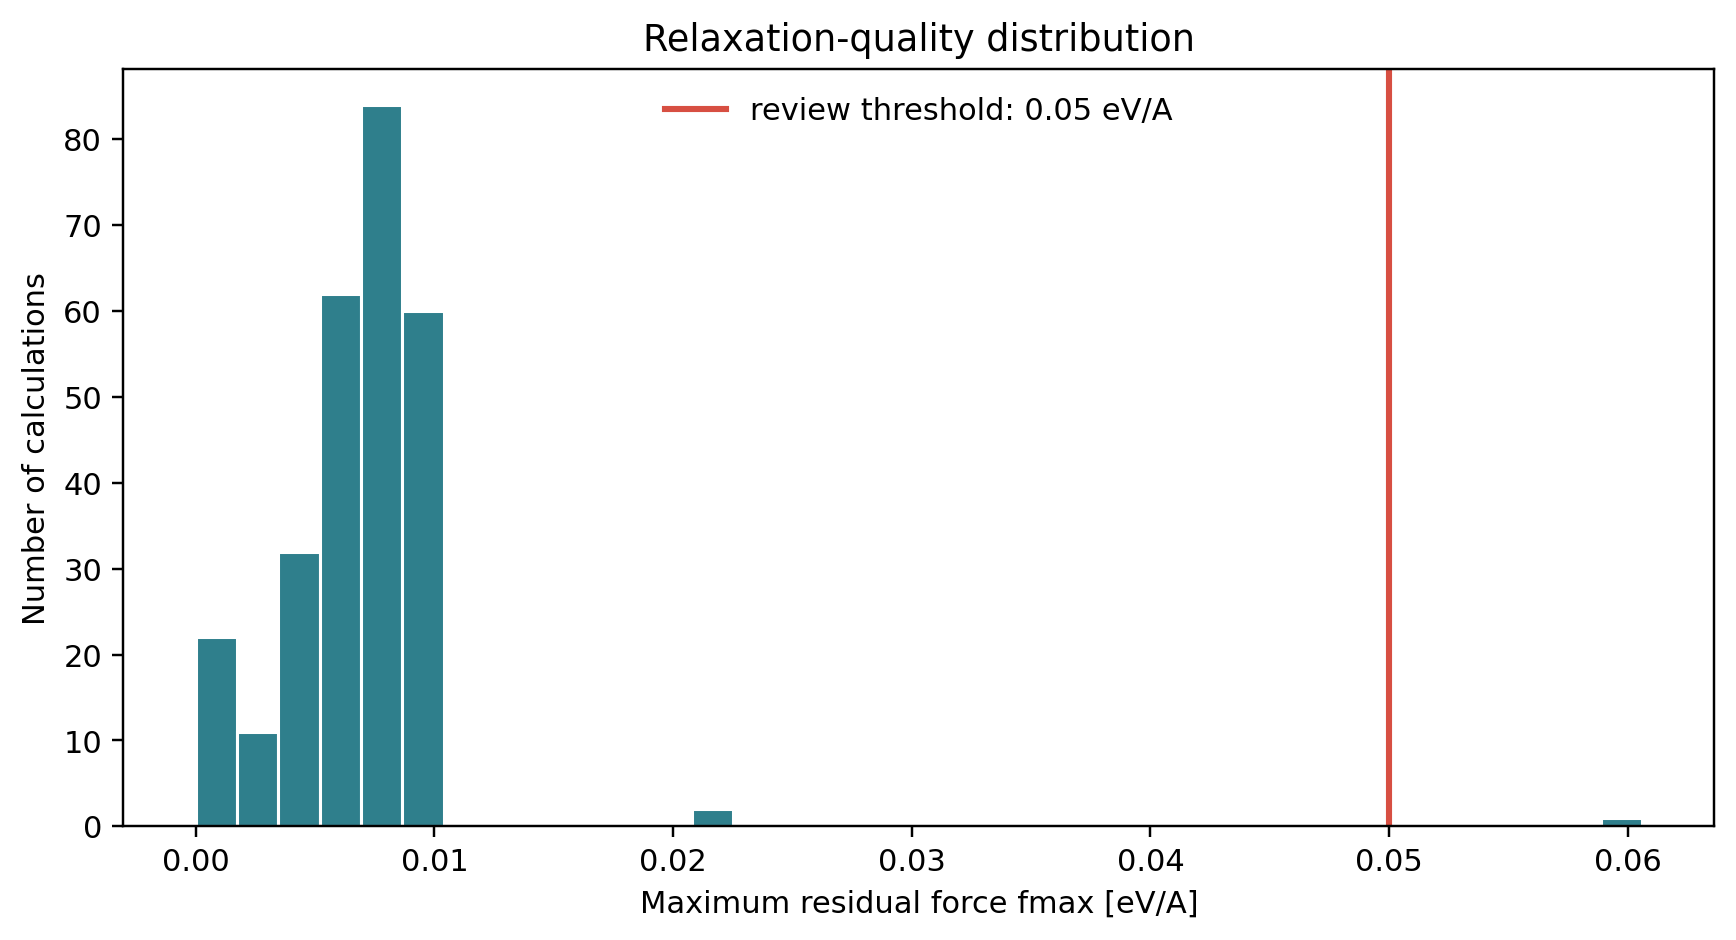
\includegraphics[width=0.78\textwidth]{fmax_distribution.png}
  \caption{Distribution of maximum residual forces in the combined Cu/Ga
  dataset. The red line marks the default review threshold used in the PFUI
  Controlroom.}
  \label{fig:fmax}
\end{figure}

\section{Bulk Phase-Diagram Algorithm}

The bulk phase diagram is computed as follows:
\begin{enumerate}
  \item define a temperature grid from 300 to 1100 K;
  \item define a gas-ratio grid from
  $\log_{10}(p_{\mathrm{H_2O}}/p_{\mathrm{H_2}})=-16$ to $4$;
  \item convert each bulk free-energy expression to a numerical function;
  \item evaluate all phase energies on the grid;
  \item select the phase with minimum energy at every grid point.
\end{enumerate}
This is equivalent to a large spreadsheet in which each cell contains the
energy of a candidate phase under one condition, and the stable phase is found
by taking the row-wise minimum across candidates.

\section{Surface Phase-Diagram Algorithm}

For each Miller index, the surface table is evaluated separately. Surface
candidates are corrected using Equation~\ref{eq:surfaceG}, normalized by area, and
compared on the same temperature/gas-ratio grid. Individual $(100)$, $(110)$,
$(111)$ and $(211)$ maps are then combined into a multi-panel view.

\chapter{Results}

\section{Bulk Energetics}

Figure~\ref{fig:bulk-energy} summarizes the bulk formation energies as a function of
Ga content. The dataset contains Cu-rich phases, intermediate Cu/Ga phases and
Ga-rich oxide-derived candidates. The wide spread in formation energy reflects
the different chemical references and thermodynamic terms represented in the
combined HDF files.

\begin{figure}[htbp]
  \centering
  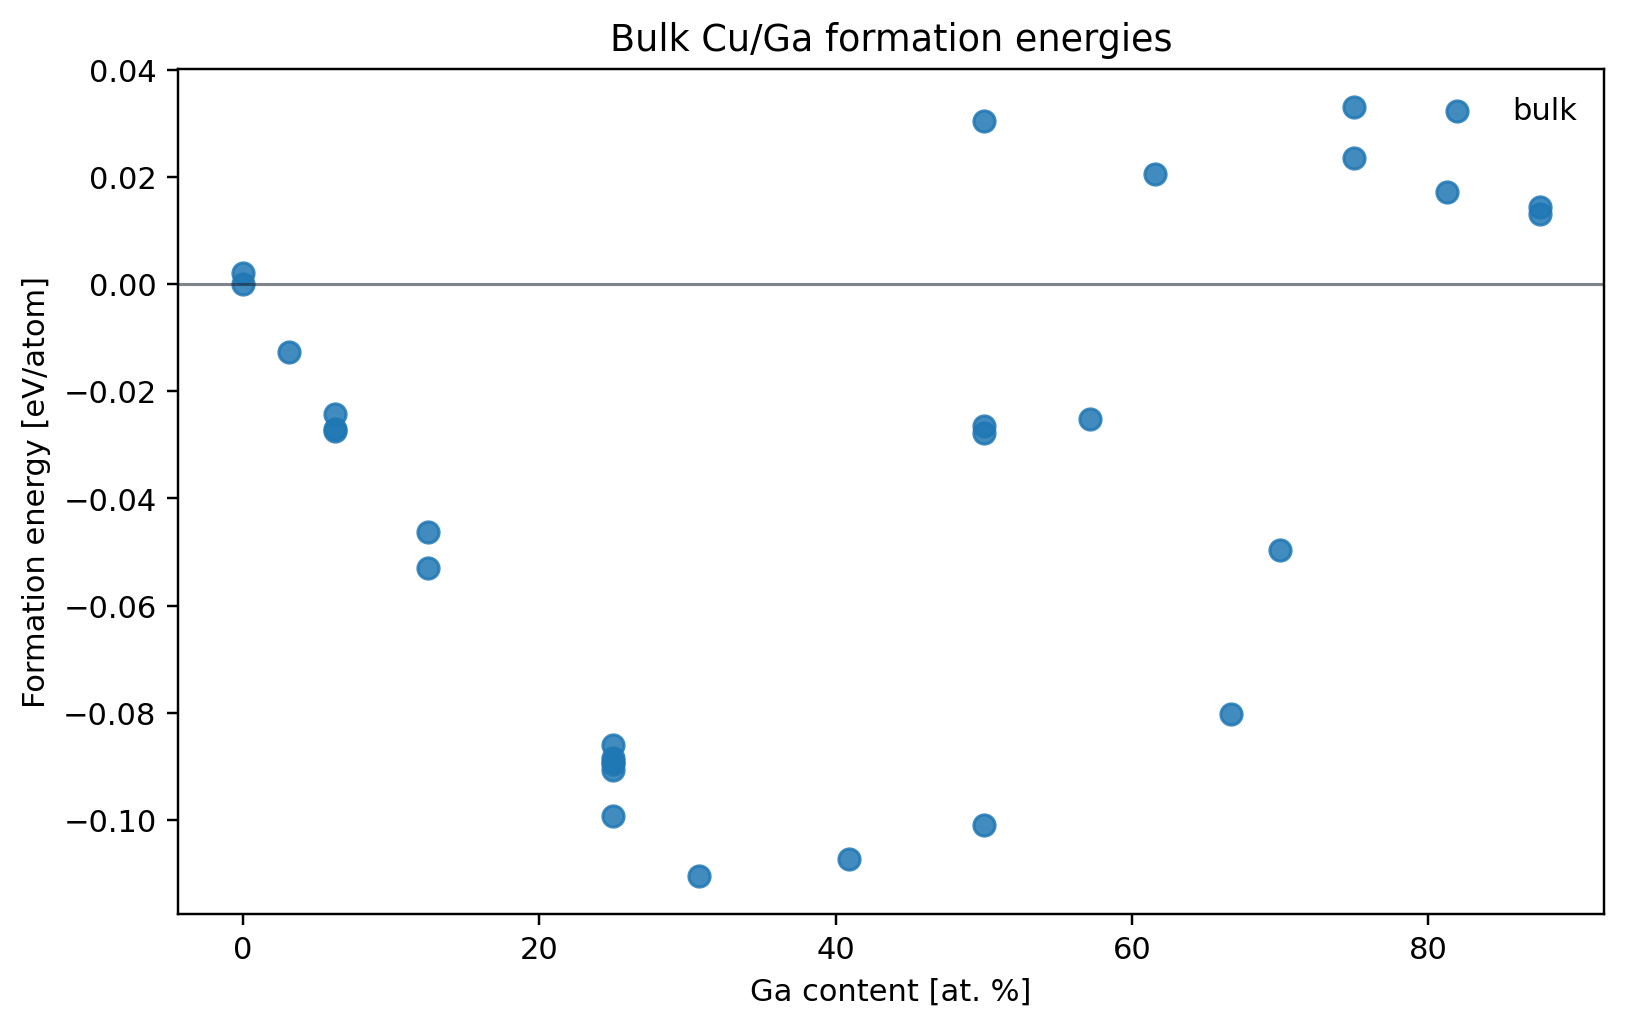
\includegraphics[width=0.78\textwidth]{bulk_energy_vs_composition.png}
  \caption{Bulk formation energies as a function of gallium content for the
  bulk and oxide-derived bulk datasets.}
  \label{fig:bulk-energy}
\end{figure}

\section{Bulk Phase Diagram}

Figure~\ref{fig:bulk-phase} shows the bulk phase map generated by the teaching
notebook. At each point of the temperature/gas-ratio grid, the color indicates
the phase with the lowest free energy. The phase fields are therefore not
fitted boundaries; they are the result of direct energy comparison across all
candidate expressions.

\begin{figure}[htbp]
  \centering
  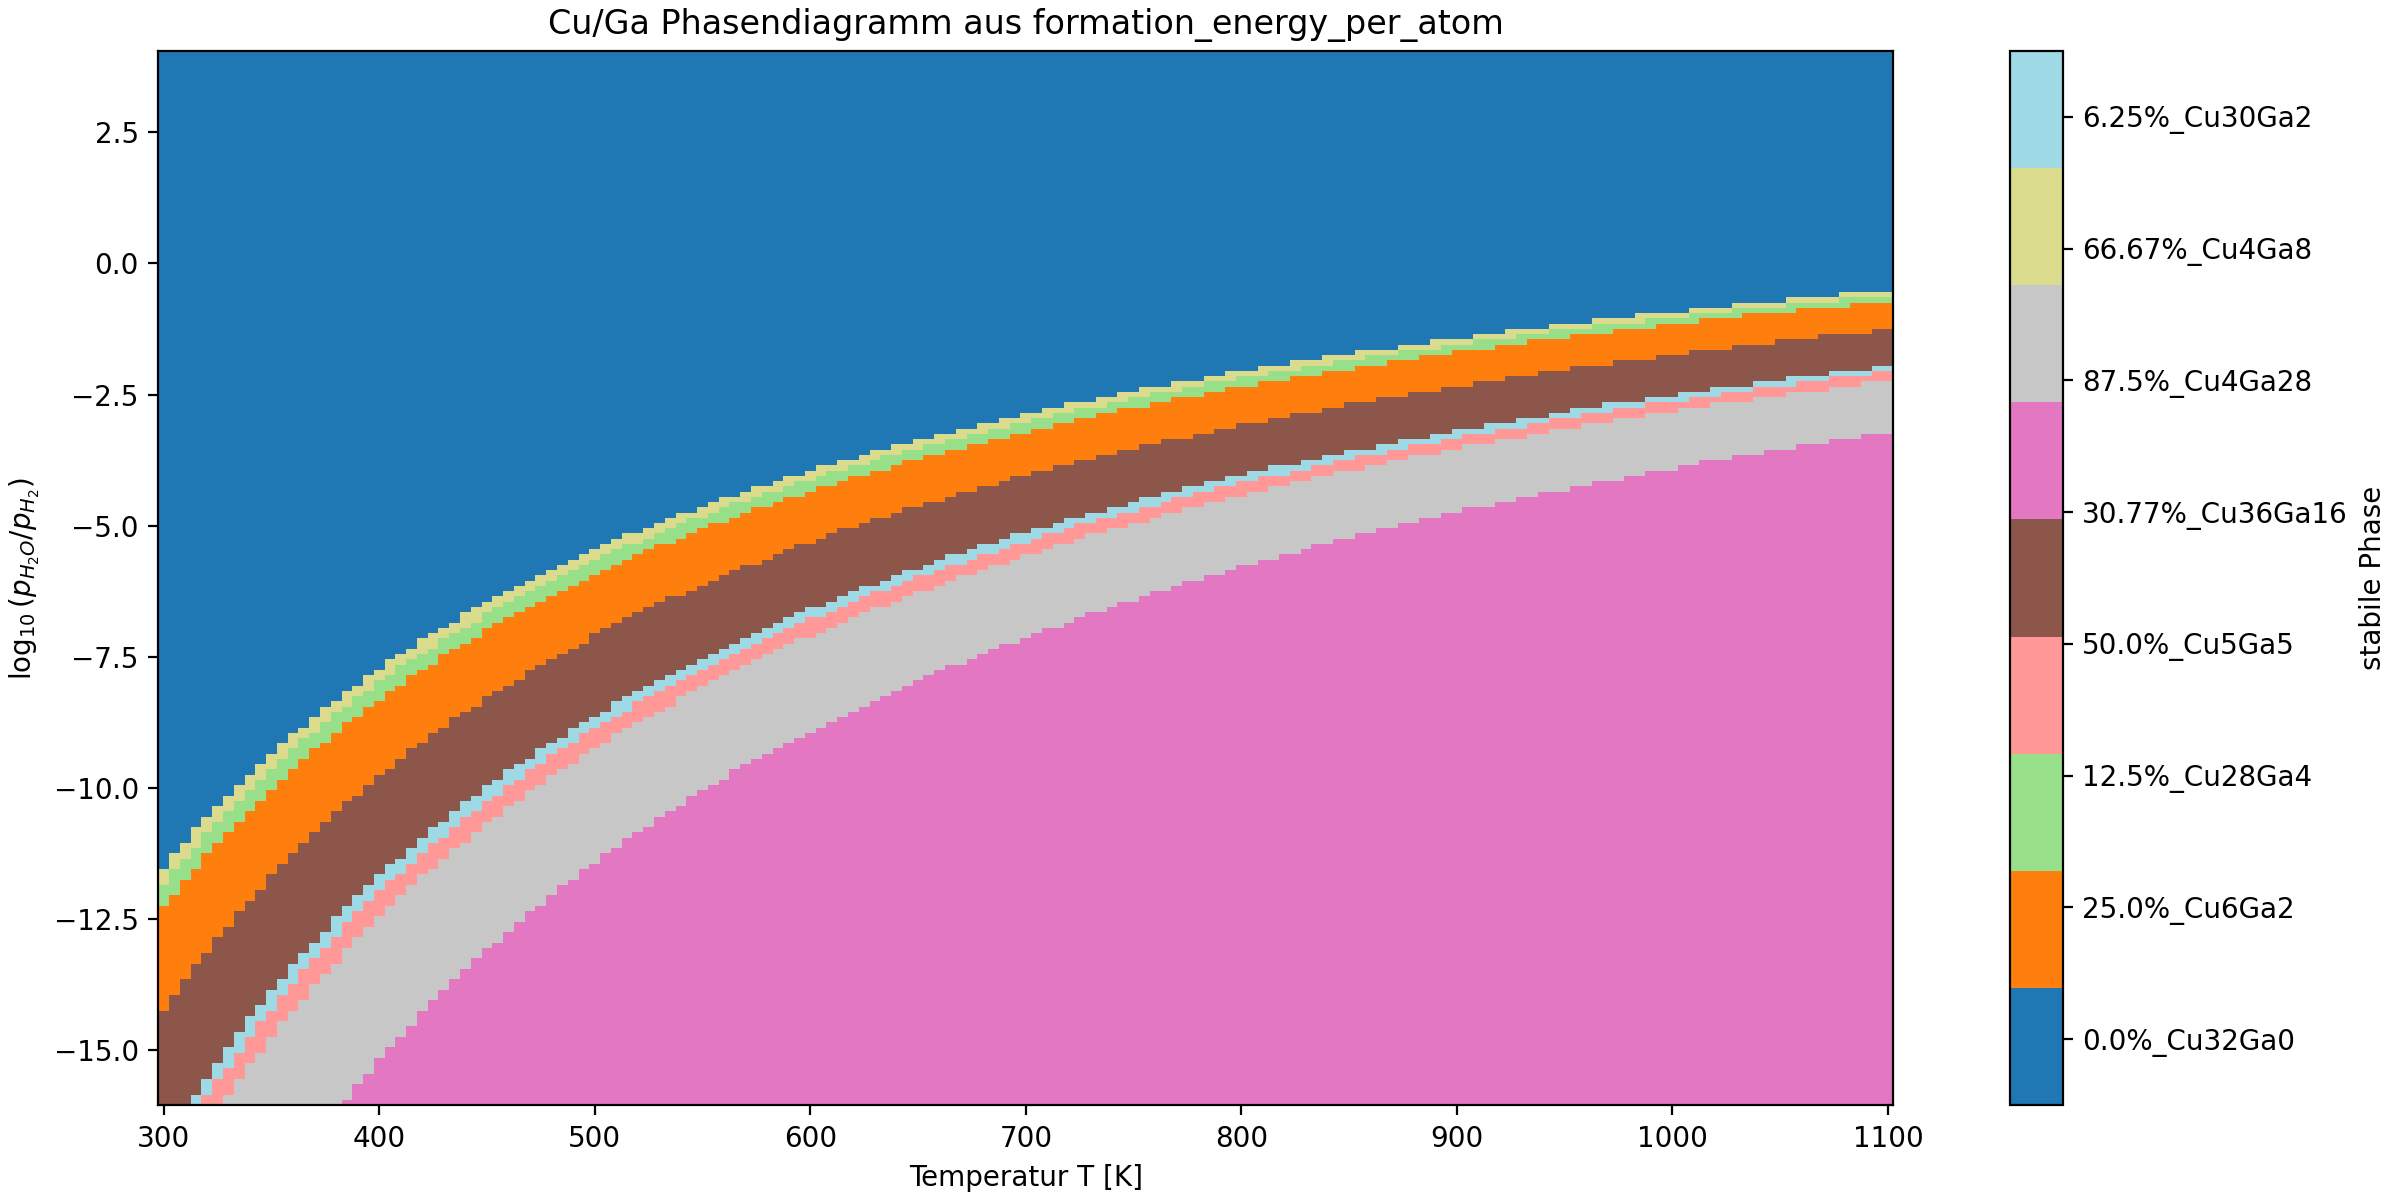
\includegraphics[width=\textwidth]{cuga_phase_diagram_2d_teaching.png}
  \caption{Bulk Cu/Ga phase diagram as a function of temperature and
  $\log_{10}(p_{\mathrm{H_2O}}/p_{\mathrm{H_2}})$. The figure is generated from
  \texttt{cuga\_muO\_temperature\_phase\_diagram.ipynb}.}
  \label{fig:bulk-phase}
\end{figure}

The largest stable bulk regions in the computed window are summarized in
Table~\ref{tab:stable-bulk}. The Cu-rich reference and a Ga-rich phase dominate
large fractions of the evaluated grid. Intermediate phases occupy smaller
transition regions.

\begin{table}[htbp]
  \centering
  \caption{Representative stable bulk phases in the computed window.}
  \label{tab:stable-bulk}
  \begin{tabular}{llrrr}
    \toprule
    Name & Formula & Ga [\%] & Stable grid [\%] & $G_\mathrm{min}$ \\
    \midrule
    Cu-bulk-Cu32 & Cu32 & 0.0 & 38.91 & 0.000 \\
    Cu-bulk-Cu4Ga28\_a & Cu4Ga28 & 87.5 & 38.30 & -4.039 \\
    Cu-bulk-CuGa2 & Cu4Ga8 & 66.7 & 7.65 & -0.379 \\
    Cu-bulk-Cu9Ga4 & Cu36Ga16 & 30.8 & 6.16 & -0.120 \\
    Cu-bulk-Cu6Ga2 & Cu6Ga2 & 25.0 & 4.70 & -0.050 \\
    \bottomrule
  \end{tabular}
\end{table}

\section{Surface Stability}

Figure~\ref{fig:surface-coverage} shows corrected surface free energies as a
function of Ga surface coverage. The comparison highlights why surface phase
diagrams must be evaluated per Miller index: the same nominal coverage does not
imply the same stability across different facets, because area, slab geometry
and reference terms differ.

\begin{figure}[htbp]
  \centering
  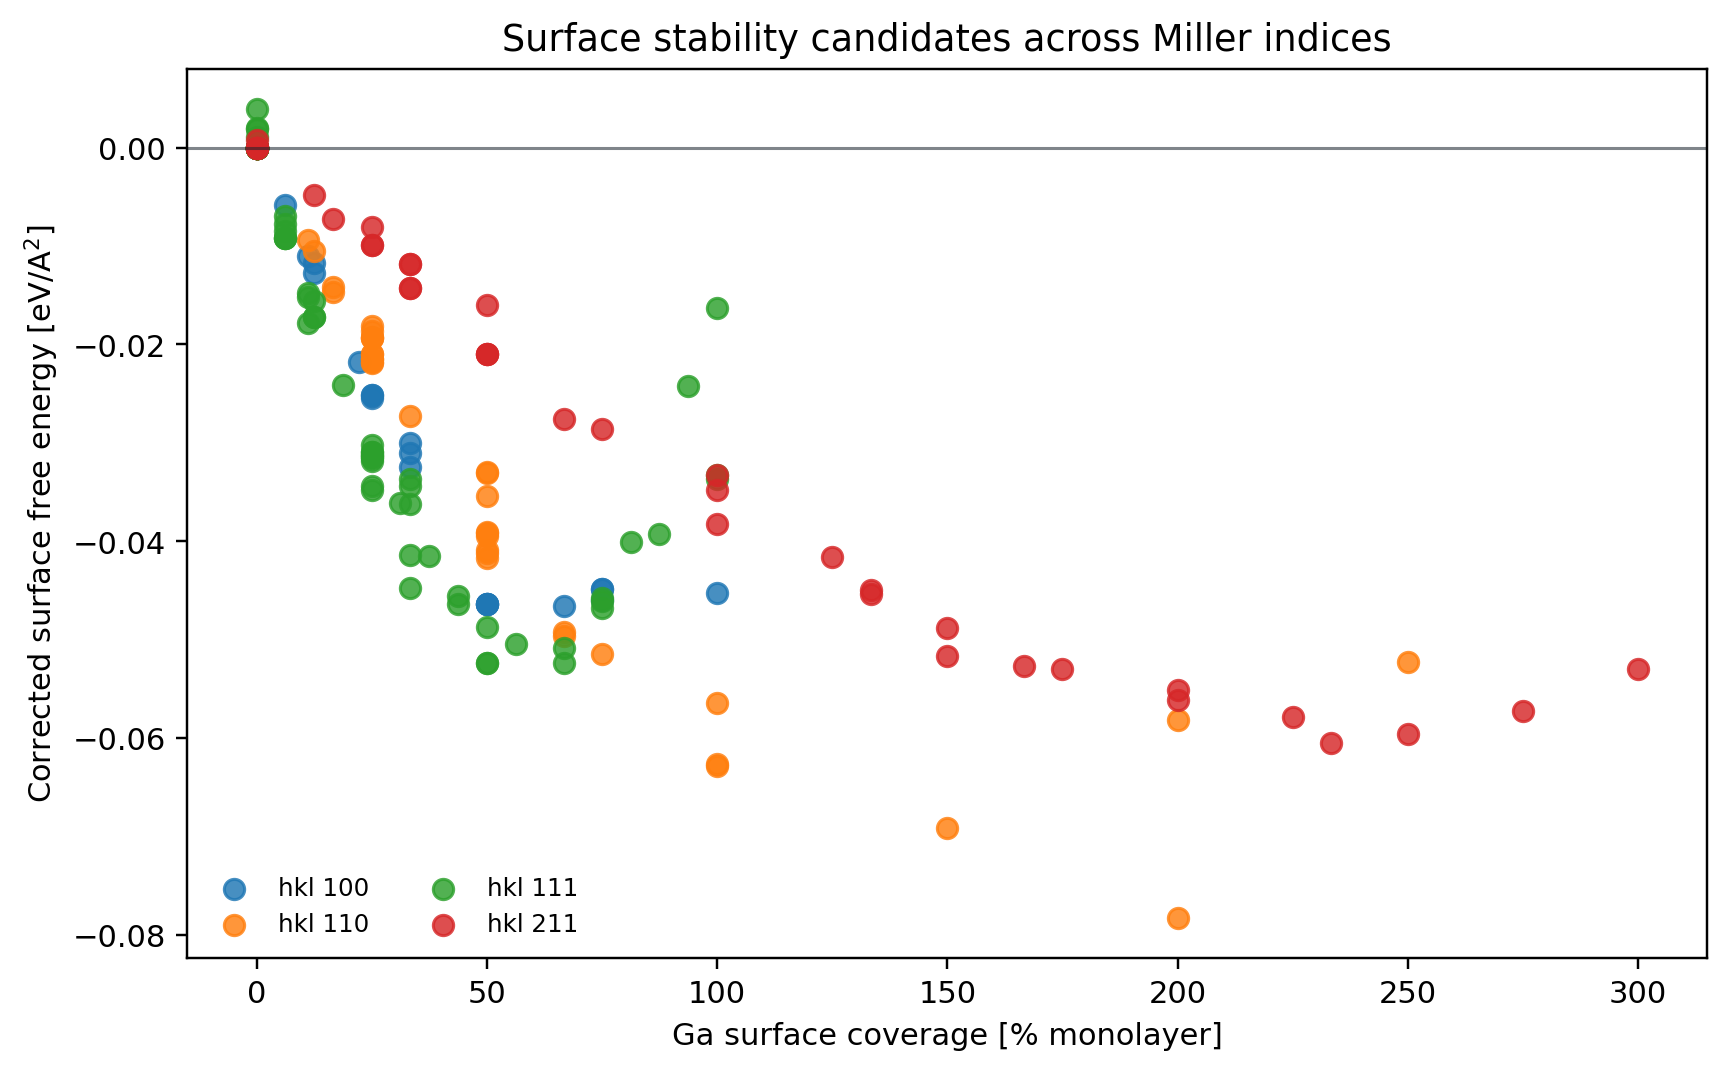
\includegraphics[width=0.82\textwidth]{surface_energy_vs_coverage.png}
  \caption{Corrected surface free energies per area as a function of Ga
  monolayer coverage for the surface datasets.}
  \label{fig:surface-coverage}
\end{figure}

The individual surface phase diagrams are shown in
Figure~\ref{fig:surface-panels}. Each panel was computed by comparing the corrected
surface free energies of candidates belonging to the same Miller index.

\begin{figure}[htbp]
  \centering
  \begin{subfigure}{0.48\textwidth}
    
\includegraphics[width=\textwidth]{cuga_surface_100_phase_diagram_2d.png}
    \caption{$(100)$}
  \end{subfigure}
  \begin{subfigure}{0.48\textwidth}
    
\includegraphics[width=\textwidth]{cuga_surface_110_phase_diagram_2d.png}
    \caption{$(110)$}
  \end{subfigure}
  \begin{subfigure}{0.48\textwidth}
    
\includegraphics[width=\textwidth]{cuga_surface_111_phase_diagram_2d.png}
    \caption{$(111)$}
  \end{subfigure}
  \begin{subfigure}{0.48\textwidth}
    
\includegraphics[width=\textwidth]{cuga_surface_211_phase_diagram_2d.png}
    \caption{$(211)$}
  \end{subfigure}
  \caption{Individual Cu/Ga surface phase diagrams for four Miller indices.
  Colors indicate the stable surface candidate at each thermodynamic condition.}
  \label{fig:surface-panels}
\end{figure}

\section{Combined Transition Fields}

Figure~\ref{fig:multiplot} combines the bulk-derived and surface-derived transition
fields in one view. This figure is useful for comparing which candidate phases
dominate the thermodynamic window and where transitions occur. The accompanying
extended CSV table stores rank, panel, phase identity, stability fraction,
temperature span, gas-ratio span and energy source.

\begin{figure}[htbp]
  \centering
  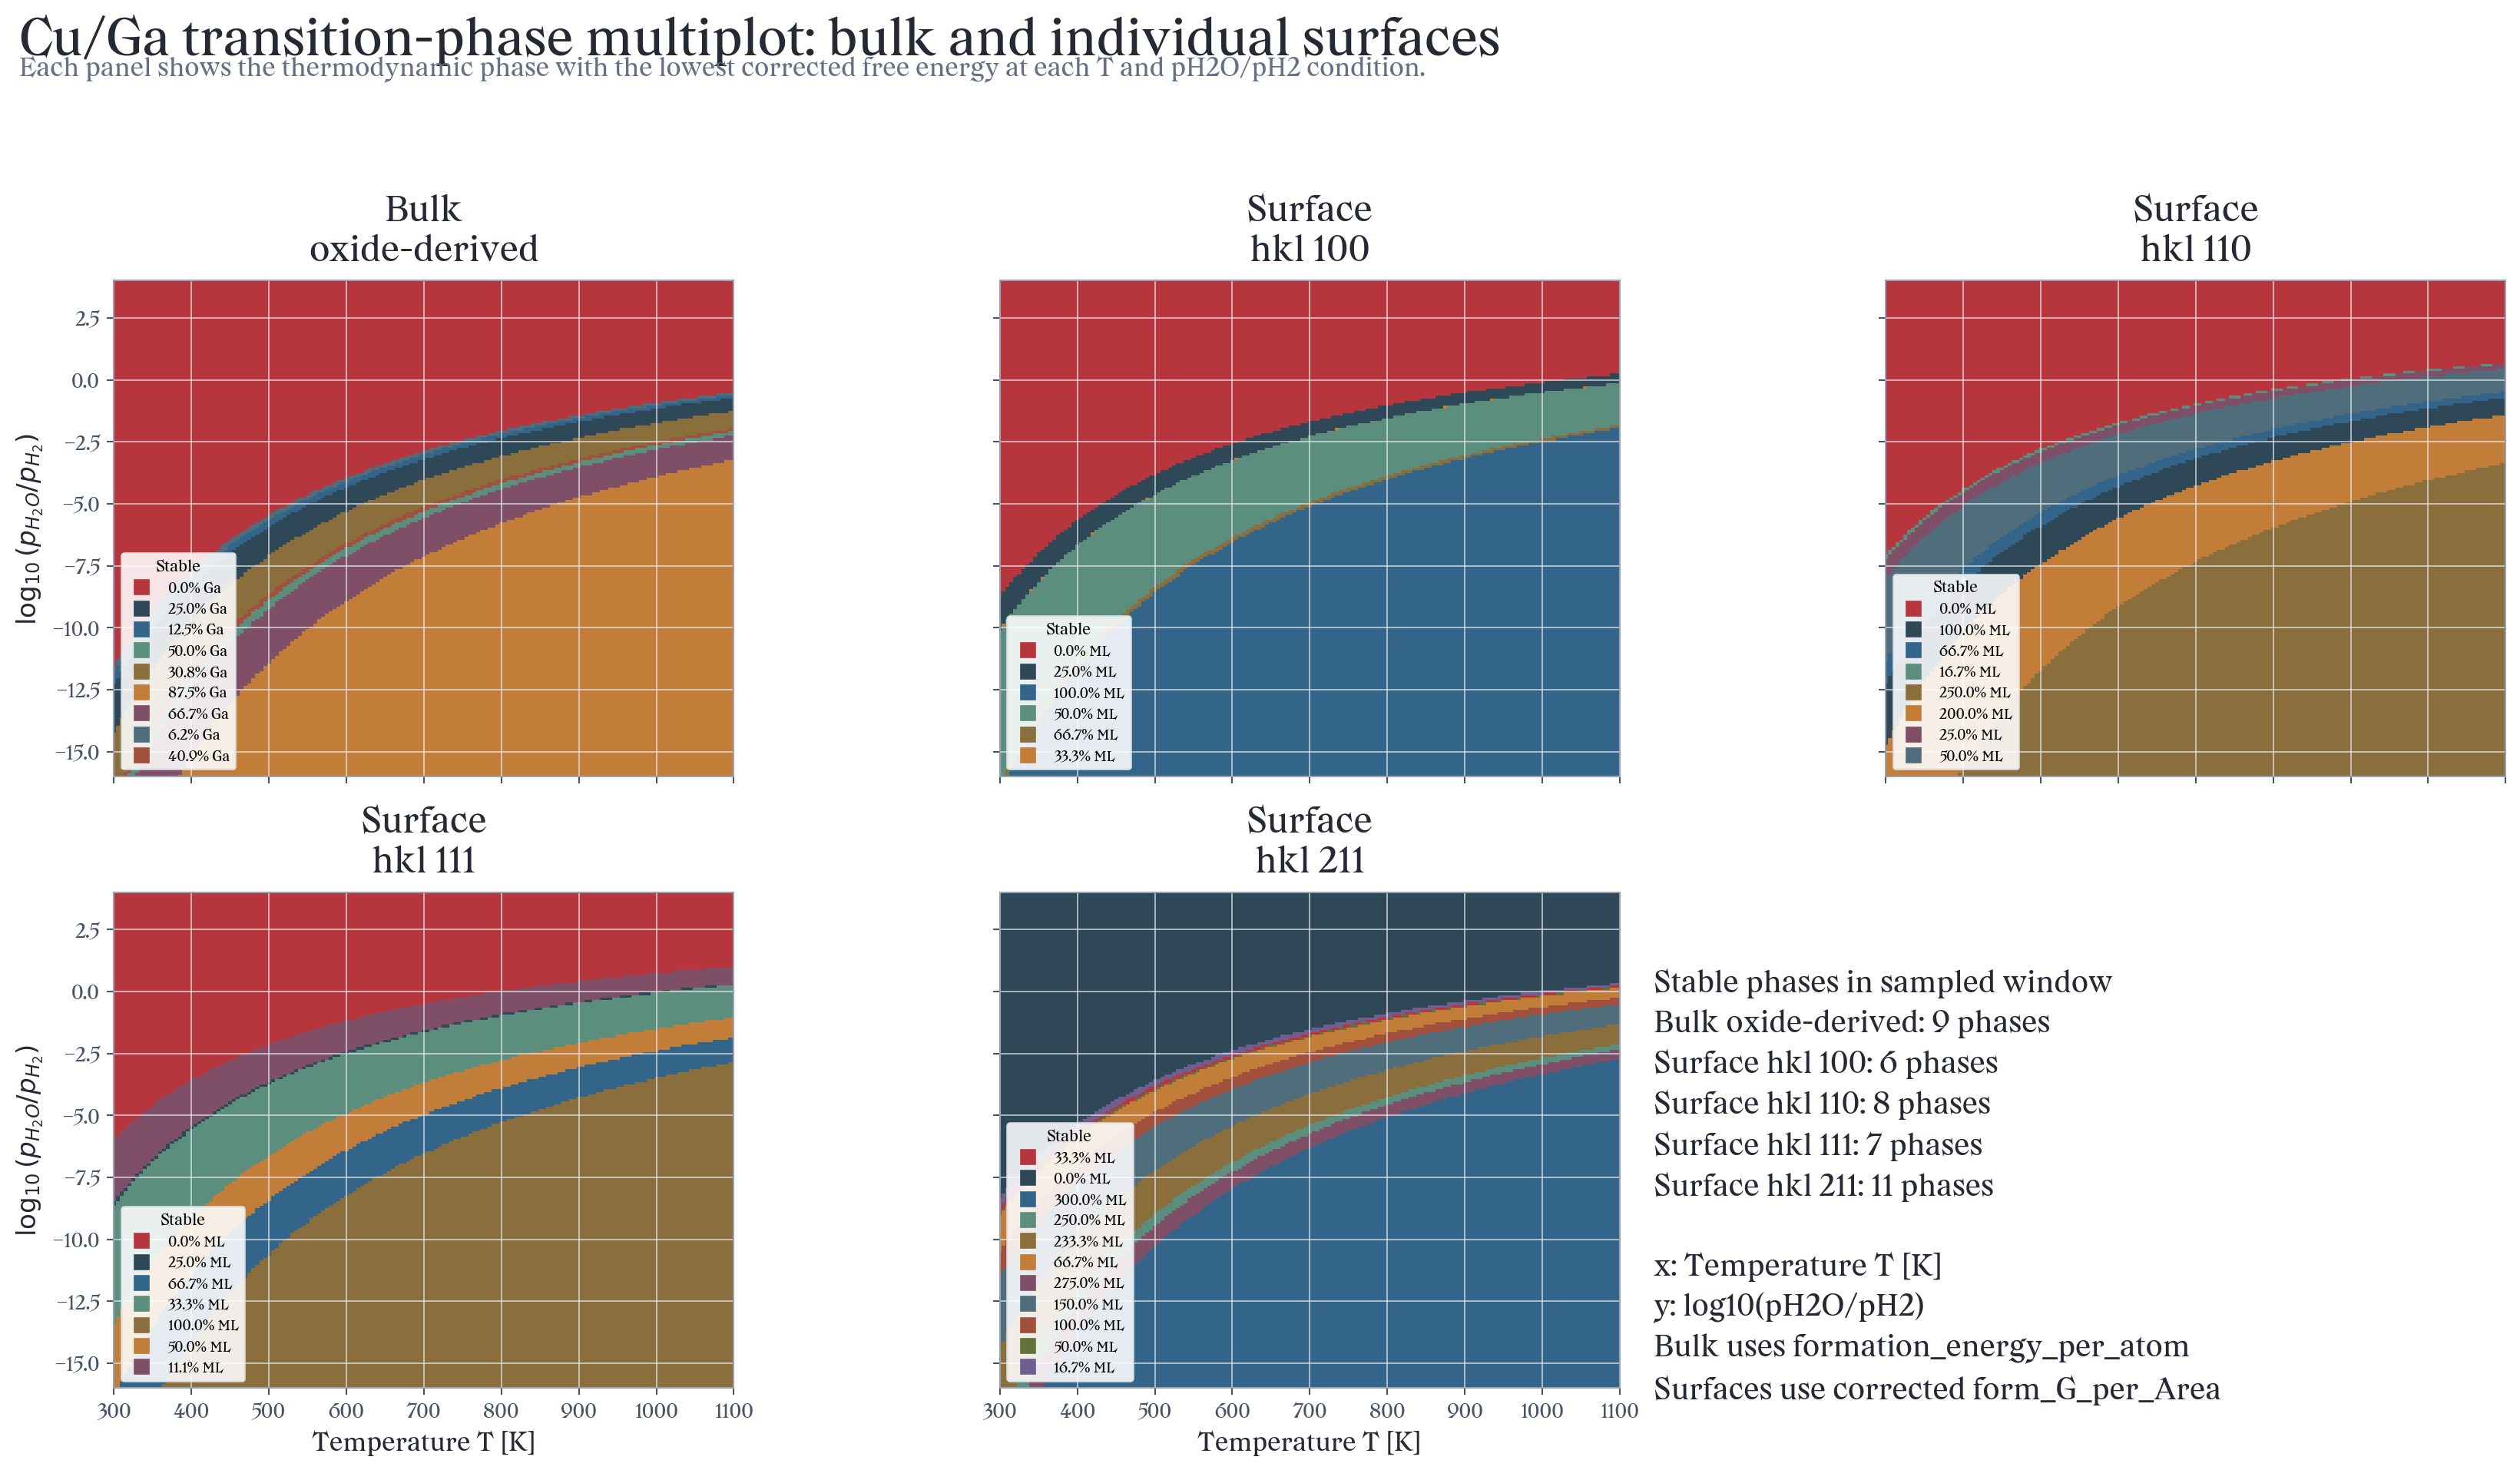
\includegraphics[width=\textwidth]{cuga_bulk_surface_transition_phase_multiplot.png}
  \caption{Combined transition-phase multiplot for bulk and surface panels.}
  \label{fig:multiplot}
\end{figure}

Figure~\ref{fig:largest-fields} ranks the largest stability fields by grid fraction.
This ranking is not a thermodynamic phase fraction; it only measures how much
of the selected computational window is occupied by a phase.

\begin{figure}[htbp]
  \centering
  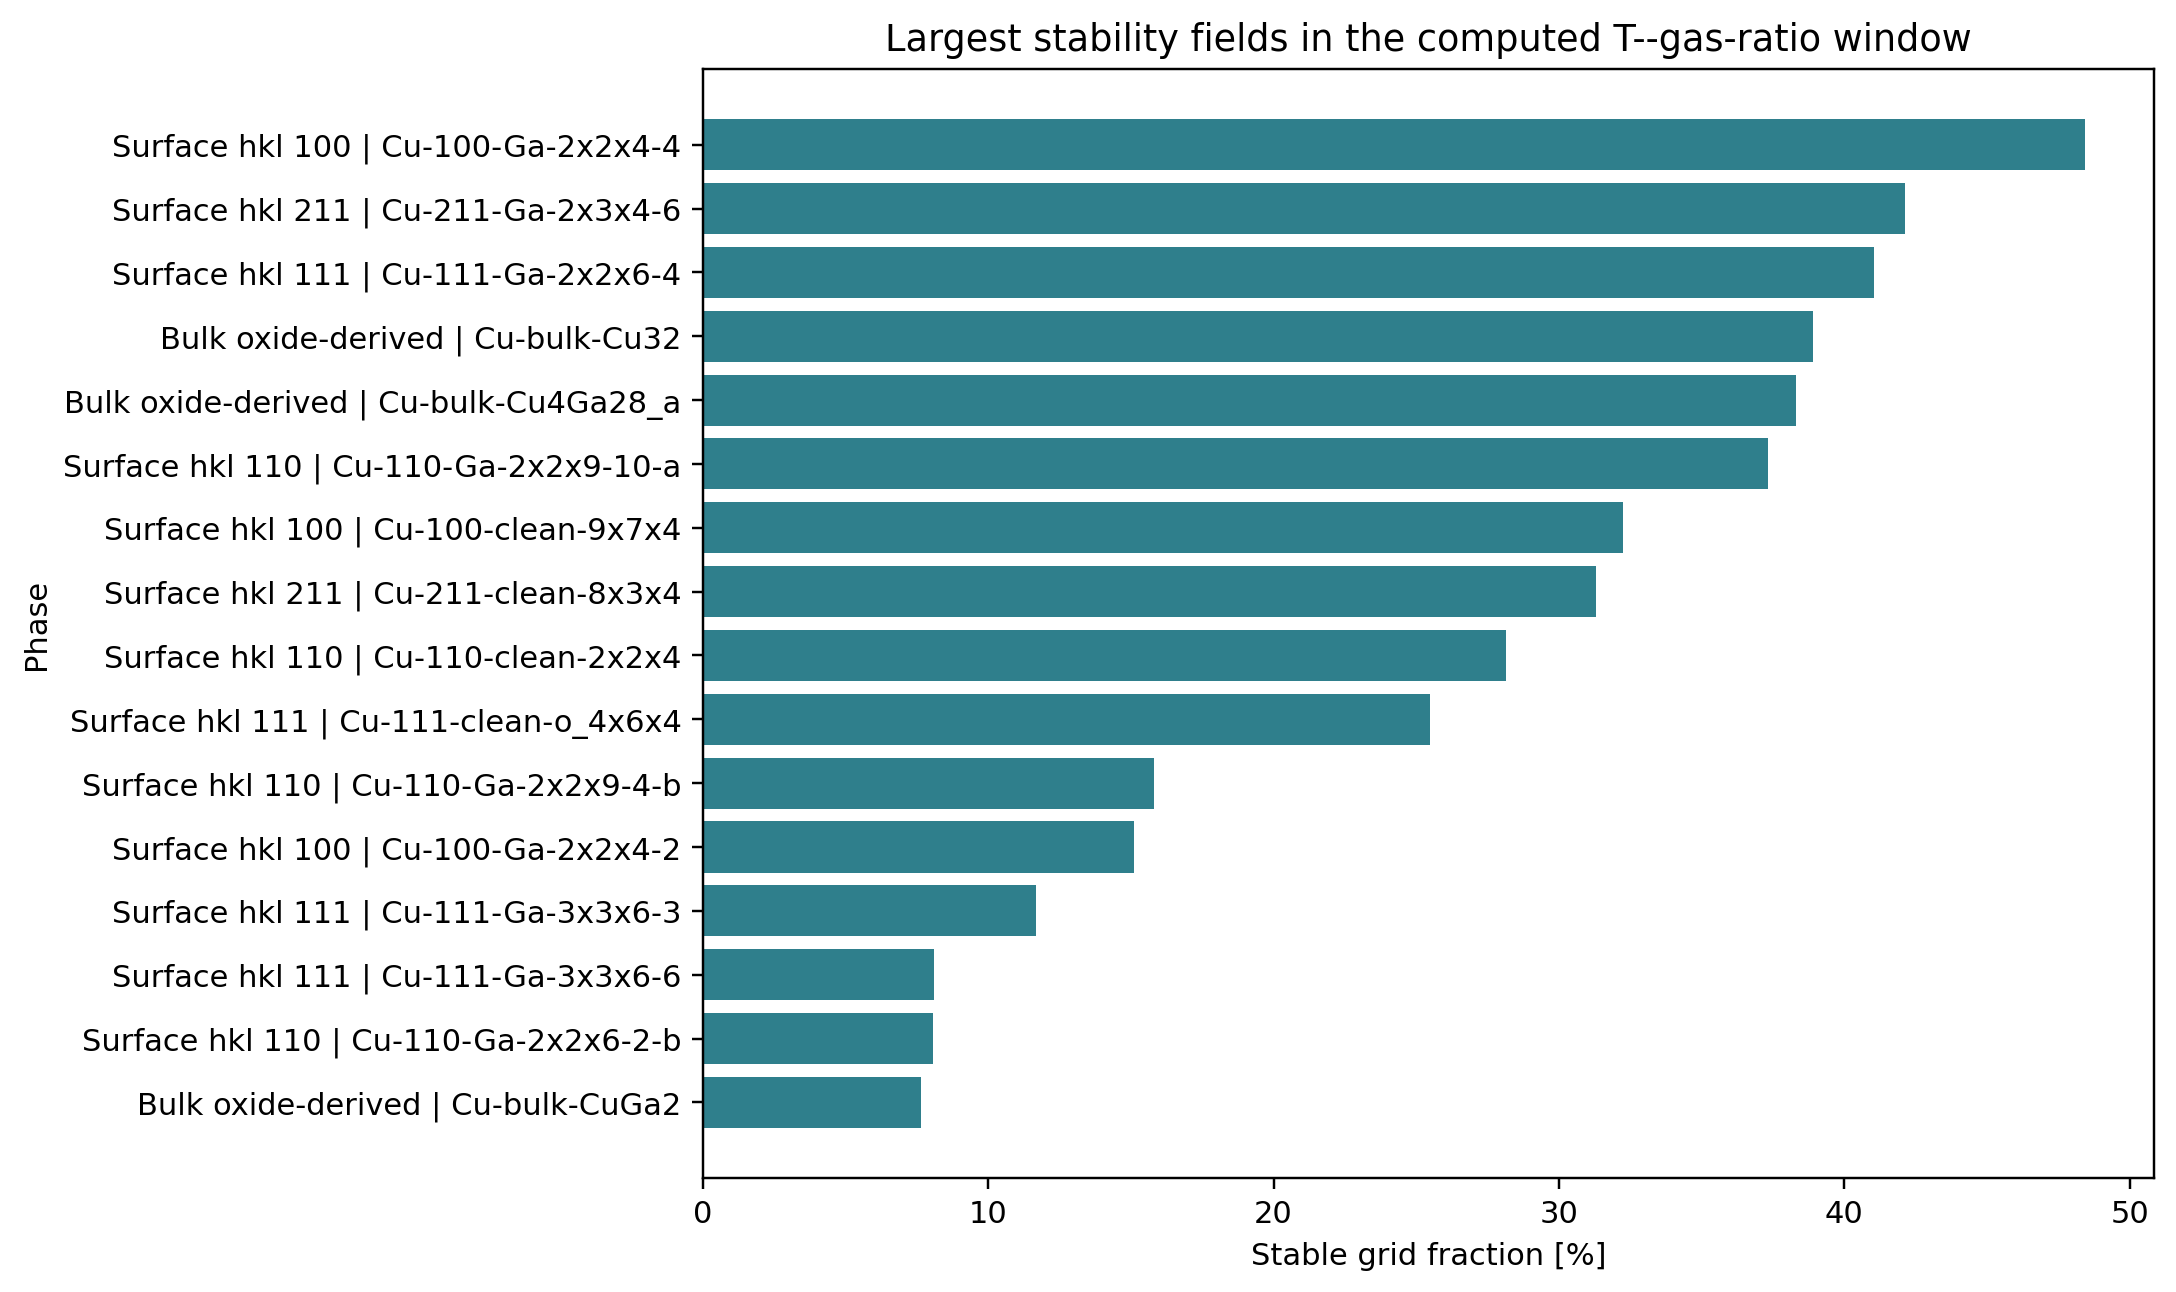
\includegraphics[width=0.95\textwidth]{largest_stable_fields.png}
  \caption{Largest stability fields in the computed temperature and gas-ratio
  window.}
  \label{fig:largest-fields}
\end{figure}

\chapter{Local User Interface Design}

\section{Motivation}

Computational chemistry datasets are rarely static. New calculations are added,
some rows become invalid, reference definitions evolve and derived energies must
be recalculated. A notebook alone is excellent for reproducibility, but less
efficient for repeated row review. PFUI was therefore developed as a local
database front end that keeps the DataFrame model visible while making common
operations clickable.

\section{PFUI Architecture}

PFUI accepts three source types:
\begin{itemize}
  \item direct pandas DataFrames;
  \item HDF files loaded with \texttt{pd.read\_hdf};
  \item OnePiece-like objects exposing \texttt{to\_dataframe()},
  \texttt{.dataframe} or \texttt{.df}.
\end{itemize}
The UI contains Records, Controlroom, Visualize and Schema tabs. The Records
tab shows row details and column profiles. The Visualize tab provides quick
scatter and histogram views. The Schema tab documents column types and samples.

\section{Controlroom Tab}

The Controlroom translates notebook operations into UI commands. It supports:
\begin{itemize}
  \item text include/exclude filters;
  \item row states: included, excluded, review and reference;
  \item materials facets such as dataset, HDF source, Miller index and slab size;
  \item numerical filters for energies, forces and surface descriptors;
  \item commands for clean references, adsorption-like rows, quality problems,
  phase-diagram candidate tables and column reviews.
\end{itemize}
This design follows the spirit of a calculation control room: rows are not
hidden by accident, and every active subset can be exported as a CSV file.

\section{Column Profiles}

The same DataFrame should not be displayed with the same columns on every page.
PFUI therefore defines column profiles for different scientific tasks:
\begin{longtable}{p{0.22\textwidth}p{0.68\textwidth}}
  \toprule
  Profile & Purpose \\
  \midrule
  Overview & identity, formula, energy and quality scan \\
  Surface Stability & surface geometry, coverage, area and corrected energies \\
  Phase Diagram & thermodynamic inputs and phase labels \\
  References & clean surfaces, bulk references and adsorption candidates \\
  Quality & convergence, force and missing-data review \\
  Structure & cell parameters, atom count and descriptor context \\
  Provenance & source HDF, source row, local path and calculation metadata \\
  \bottomrule
\end{longtable}

\chapter{Future Adsorption-Energy Workflow}

The next planned workflow is adsorption-energy analysis. For a target
adsorbate--surface row, an adsorption energy can be expressed as
\begin{equation}
  E_\mathrm{ads}
  =
  E_{\mathrm{adsorbate+surface}}
  -
  E_{\mathrm{clean~surface}}
  -
  n_{\mathrm{ads}}E_{\mathrm{adsorbate~reference}}.
  \label{eq:eads}
\end{equation}
The key database challenge is reference resolution. The clean reference surface
should be found from the same dataset, preferably by matching the \texttt{Name}
column, Miller index, slab size and composition. PFUI therefore already derives
\texttt{reference\_role}, \texttt{reference\_key},
\texttt{is\_clean}, \texttt{is\_adsorbate\_like} and
\texttt{adsorbate\_guess}.

Ambiguous references should not be accepted silently. If multiple clean
surfaces match one adsorbate row, the UI should mark the row as
\texttt{review}. This is important because a wrong reference can shift
adsorption energies by much more than typical trends between surface sites.

\chapter{Conclusions}

This thesis demonstrates a local computational chemistry workflow for Cu/Ga
bulk and surface datasets stored in OnePiece-style pandas HDF files. The data
were combined into a 274-row working database, enriched with context columns and
used to compute thermodynamic phase diagrams across temperature and
$p_{\mathrm{H_2O}}/p_{\mathrm{H_2}}$. Bulk and surface candidates show distinct
stability fields, and the surface analysis confirms that each Miller index must
be treated individually.

Beyond the numerical phase diagrams, the work emphasizes the importance of
local database usability. The PFUI prototype provides a bridge between
notebooks and a research database interface. It allows calculation rows to be
filtered, reviewed, marked as references or excluded, and exported for further
analysis. The column-profile design reduces cognitive load by showing the
columns relevant to the current scientific task rather than presenting all
available metadata at once.

The resulting workflow is reproducible, local and extensible. It is ready for
future adsorption-energy calculations in which clean surfaces and molecular
references are resolved directly from the dataset and every derived energy can
be traced back to the source HDF rows.

\appendix

\chapter{Reproducibility Notes}

The main thesis figures were generated with:
\begin{verbatim}
python thesis/build_thesis_figures.py
\end{verbatim}

The source notebooks are located in:
\begin{verbatim}
notebooks/
notebooks/onepiece_phase_tutorial/
\end{verbatim}

The combined PFUI dataset cache is:
\begin{verbatim}
notebooks/phase_diagram_outputs/cuga_full_dataset.pkl
\end{verbatim}

The PFUI app for browsing the complete local dataset is launched with:
\begin{verbatim}
python3 -m streamlit run examples/cuga_full_streamlit.py \
  --server.headless true --server.port 8502
\end{verbatim}

\chapter{Important Generated Files}

\begin{itemize}
  \item \texttt{thesis/main.tex}: this thesis.
  \item \texttt{thesis/build\_thesis\_figures.py}: figure-generation script.
  \item \texttt{thesis/figures/}: figures used by the thesis.
  \item \texttt{thesis/tables/}: CSV tables used for summaries.
  \item \texttt{src/pfui/materials\_columns.py}: column-profile and derived
  descriptor logic.
\end{itemize}

\bibliographystyle{unsrt}
\bibliography{references}

\end{document}
